\section{问题三：共享 FIFO 缓存下的多处理器调度}
\subsection{缓存状态与双带宽事件模型}
问题三继承场景 B 的合法方案集 $\mathcal P_B(k)$、跨核释放与核内内存约束，新增容量为 $C$ 的共享只读 L2。它不是每核各有一份，也不改变已生成的逻辑 COPY 数量。对时刻 $t$ 按进入先后排序的逻辑张量队列记为 $Q(t)$，有
\begin{equation}\label{eq:q3-capacity}
\sum_{x\in Q(t)}s_x\le C,\qquad C=1\,048\,576\ {\rm bytes}.
\end{equation}
正字节 \texttt{COPY\_IN} 事件 $e$ 在发射时刻 $a_e$ 查询逻辑张量标识。若标识已在 $Q(a_e^-)$ 中则 $h_e=1$，改由 L2 服务；否则 $h_e=0$，仍由 DDR 服务。命中不刷新 FIFO 次序。搬运在完成时按官方处理顺序进行填充：未驻留且大小不超过 $C$ 的张量，从队首淘汰至有足够空间后入队；超容量张量旁路。两个同时发射的冷读不能因为较早一个尚在途中而合并为一次命中。完成时的重新插入、相同时间事件次序等均保持官方语义。

设 $A_D(t),A_L(t)$ 分别为 DDR 和 L2 池的在途操作集合，$b_D=60$、$b_L=250$ bytes/cycle。每条搬运按所属池的独占带宽形成初始服务工作量，活跃集合不变的时间段内，各自池内公平分享服务：
\begin{equation}\label{eq:q3-service}
\dot w_e(t)=-\frac{1}{|A_r(t)|},\qquad
e\in A_r(t),\quad r\in\{D,L\}.
\end{equation}
事件到达或完成后须结算剩余工作并重算完成时刻；实际评价还依官方整数周期取整。两池独立，不能把 $60+250$ 当作共同带宽，也不能给每个核心各分配一条 $250$ bytes/cycle 的 L2 通道。L2 命中只改变 COPY 的服务池，不能绕过 \eqref{eq:q2-release} 中的跨核同步，不能占用别的 Pipe 插队，亦不能使超出 L1/UB 的物理实例合法。

于是问题三在相同合法方案集上求
\begin{equation}\label{eq:q3-objective}
\min_{p\in\mathcal P_B(k)}
\operatorname{lex}\bigl(T_i^{L2}(p;C,b_L),D_i(p)\bigr).
\end{equation}
字节命中率为
\begin{equation}\label{eq:q3-hit}
H_i=\frac{\sum_{e:\ {\rm COPY\_IN},\ s_e>0}h_es_e}
{\sum_{e:\ {\rm COPY\_IN},\ s_e>0}s_e}.
\end{equation}
分母为零时只在统计程序中定义为零并标注“无有效读取”。官方命中率按字节而非按次数统计。$D_i$ 是插入额外逻辑 COPY 的字节量，不因命中自动扣减；同一方案分别在无 L2 和 L2 下评价，该字段应相同。命中字节可作为实际 DDR 服务减量的辅助诊断，但 $H_i$ 越高未必总周期越短，因为同步、计算、L2 带宽竞争以及关键路径变化仍可能占主导。

\subsection{缓存微事件及状态转移的完整定义}
问题三的方案空间仍是满足场景 B 合法性条件的 $\mathcal P_B(k)$，并未新增“选择某张量是否命中”的自由变量。命中由方案诱导的 COPY 发射时刻与全核共享 FIFO 状态内生决定。为区别实际缓存与外层预测，以离散事件序号 $j$ 表示官方确定的同刻处理顺序，记
\begin{equation}\label{eq:q3-cache-state}
Q_j=(x_1,\ldots,x_{m_j}),\qquad
u_j=\sum_{r=1}^{m_j}b_{x_r}\le C,\qquad Q_0=\varnothing .
\end{equation}
队列从左至右按\emph{进入缓存的先后}排序，$C=1\,048\,576$ bytes。对正字节 \texttt{COPY\_IN} 事件 $e$，在\emph{发射}时读取其逻辑张量标识 $\ell_e$，确定
\begin{equation}\label{eq:q3-lookup}
h_e=\mathbf 1\{\ell_e\in Q_{j(e)^-}\},\qquad
r(e)=
\begin{cases}
L,&h_e=1,\\
D,&h_e=0,
\end{cases}
\end{equation}
其中 $L,D$ 分别是 L2 与 DDR 服务池。查询命中不把张量移到队尾，这与最近最少使用策略不同。服务池在发射时已经确定；即使传输在途期间该张量被别的完成事件淘汰，本次请求也不临时改道。对于非正字节读取与 COPY\_OUT，按官方特殊规则执行，但不把它们计入“正字节读入命中率”的分子或分母。

填充发生在读入\emph{完成}时。令事件完成的逻辑张量为 $x$。若标识无效、$b_x>C$ 或 $x$ 已在 $Q_j$ 中，队列保持；否则选择最短的队首淘汰前缀长度
\begin{equation}\label{eq:q3-fifo-evict}
h^\star=\min\left\{h\in\{0,\ldots,m_j\}:
u_j-\sum_{r=1}^{h}b_{x_r}+b_x\le C\right\},
\end{equation}
再定义
\begin{equation}\label{eq:q3-fifo-next}
Q_{j+1}=(x_{h^\star+1},\ldots,x_{m_j},x),\qquad
u_{j+1}=u_j-\sum_{r=1}^{h^\star}b_{x_r}+b_x .
\end{equation}
对于 $b_x\le C$，取 $h=m_j$ 总能容纳，故式\eqref{eq:q3-fifo-evict}的集合非空。式\eqref{eq:q3-fifo-next}是 FIFO：只删除队首前缀，幸存者相对次序不变，新张量放队尾。原先命中的在途读取若在完成前被淘汰，完成时若缓存中仍无该逻辑张量，也按相同规则重新插入；若已由别的完成事件插入，则不刷新队列。两个几乎同时发射的冷读在尚无完成填充时均可未命中，不能为了提高命中率私自合并。

这些规则给出三个可证明的不变量。首先，$Q_0$ 不含重复标识，插入前先判驻留，故归纳可得所有 $Q_j$ 中标识唯一。其次，$b_x>C$ 的张量旁路，其他新入张量按式\eqref{eq:q3-fifo-evict}淘汰到足够空间，所以 $0\le u_j\le C$ 恒成立。第三，命中只读取、不重排，淘汰只删前缀，故幸存张量的 FIFO 相对顺序保持。由发射时的二值判定，每个有合格逻辑键的正字节读取恰好计入命中或未命中之一。这是实现缓存事件账本时的局部校验条件，也说明只按访问频次估算 L2 收益会遗漏顺序与在途状态。

\subsection{两个共享服务池及命中率}
问题三保留共享 DDR 总带宽 $b_D=60$ bytes/cycle，并新增\emph{全核共同}的 L2 读带宽 $b_L=250$ bytes/cycle。两条带宽属于不同池；一个 L2 命中请求不能同时按 DDR 与 L2 服务，也不能把两者相加为一个 310 bytes/cycle 的通用资源。对事件 $e$ 的正字节 $b_e$，定义独占参考服务工作量
\begin{equation}\label{eq:q3-exclusive-work}
q_e^r=\left\lceil\frac{b_e}{b_r}\right\rceil,
\qquad r\in\{D,L\}.
\end{equation}
在活跃集合不变时各池分别按式\eqref{eq:q3-service}分享，事件到达或完成后结算剩余工作，再由官方的整数事件顺序决定下一次状态转移。整数上取整、零字节请求及同刻多个完成事件的处理可以改变下一次发射与 FIFO 次序，故这里的连续服务式是物理解释，精确主结果仍取官方事件仿真。

令 $R(p)=\sum_{e\in\mathcal R_{\rm in}(p)}b_e$ 为固定方案下所有合格正字节读入量，$X(p)$ 为其余必须经 DDR 的逻辑搬运量，$H(p,C,b_L)=\sum_e h_e b_e$ 为命中字节。固定方案展开的 COPY 集合不因只读 L2 本身改变，因此两池的字节工作量可写成
\begin{equation}\label{eq:q3-pool-bytes}
D_D=X+R-H,\qquad D_L=H,\qquad
H_B=
\begin{cases}
H/R,&R>0,\\
0\text{（标记为无有效读取）},&R=0 .
\end{cases}
\end{equation}
$H_B$ 是字节命中率，不是命中请求次数除以请求总次数。式\eqref{eq:q3-pool-bytes}还说明：命中会改变\emph{由哪个服务池承担}读取，却不自动删除方案中的逻辑 COPY 事件。因此同一个 $p$ 在 B 与 L2 两种硬件环境下评价，逻辑额外搬运 $D(p)$ 应相同，虽然实际 DDR 服务字节可减少。若缓存感知搜索最终改用另一个 $p_L$，其划分和通信本身改变，$D(p_L)$ 则可能升高。

仅由共享带宽的容量限制可得
\begin{equation}\label{eq:q3-two-pool-bound}
T^{L2}(p)\ge
\max\left\{\frac{X+R-H}{b_D},\frac{H}{b_L}\right\}.
\end{equation}
两项取最大而非相加，因为两个服务池可并行运行，计算 Pipe 也可与两者重叠。若只观察 $H_B$ 增加，式\eqref{eq:q3-two-pool-bound}的 DDR 项下降，但 L2 项上升，且真实关键路径可能转移；“命中率升高必然缩短 Makespan”不成立。对于完成时间的更强条件界，还可与式\eqref{eq:universal-compute-bound}、固定方案每核计算 Pipe 负载取最大；这些界不能反推出真实完成时间等于各资源忙碌时长之和。

\subsection{乐观命中上限与容量、带宽包络}
对固定方案 $p$，设逻辑张量 $x$ 被正字节读取 $m_x\ge1$ 次、每次大小为 $b_x$。空缓存必须经历至少一次冷读；$b_x>C$ 的张量根本不能驻留。因此无需知道访问次序便有乐观上限
\begin{equation}\label{eq:q3-hit-upper}
0\le H\le H_{\max}(p,C)=
\sum_{x:\,b_x\le C}(m_x-1)b_x.
\end{equation}
等号通常难达到：并发冷读可能多次未命中，不同张量之间的 FIFO 淘汰也可能让已读张量再次变冷。式\eqref{eq:q3-hit-upper}只回答“最多有多少重复读取字节有资格转向 L2”，并不保证这些字节真实命中。

为了说明硬件收益的\emph{理论边界}而非预测实测，将 $H$ 放宽为区间 $[0,H_{\max}]$ 内可任意选择的连续变量 $z$。对固定 $p$ 的两池负载，构造
\begin{equation}\label{eq:q3-relaxed-envelope}
\Phi(p;C,b_L)=
\min_{0\le z\le H_{\max}(p,C)}
\max\left\{\frac{X+R-z}{b_D},\frac{z}{b_L}\right\}.
\end{equation}
第一项随 $z$ 下降，第二项随 $z$ 上升，其无约束交点解由
\[
\frac{X+R-z}{b_D}=\frac{z}{b_L}
\quad\Longrightarrow\quad
z_0=\frac{(X+R)b_L}{b_D+b_L}.
\]
由于 $z_0\ge0$，受上限截断后的最优放宽值为
\begin{equation}\label{eq:q3-envelope-optimum}
z^\star=\min\{H_{\max}(p,C),z_0\},\qquad
\Phi(p;C,b_L)
=\max\left\{\frac{X+R-z^\star}{b_D},\frac{z^\star}{b_L}\right\}.
\end{equation}
真实 $H$ 必在放宽区间中，故 $\Phi(p;C,b_L)\le T^{L2}(p)$。容量 $C$ 增大时 $H_{\max}$ 不减，放宽可行域扩大；带宽 $b_L$ 增大时，对于每个 $z$ 的第二项不增，所以 $\Phi$ 对两参数均不增。这是\emph{乐观包络}的单调性，不是 FIFO 真实周期的单调性证明。真实队列与完成顺序会随容量、带宽改变，甚至使某个固定方案在带宽增大时略慢。

全空间最优值也必须与有限候选和方案条件界分开。定义
\begin{equation}\label{eq:q3-optimality-sandwich}
T^\star=\min_{p\in\mathcal P_B(k)}T^{L2}(p),\qquad
U_{\mathcal A}=\min_{p\in\mathcal A}T^{L2}(p),
\end{equation}
其中 $\mathcal A\subset\mathcal P_B(k)$ 是实际完成官方评价的有限集合。由式\eqref{eq:universal-compute-bound}和集合包含关系，严格成立
\begin{equation}\label{eq:q3-bound-order}
L_0(k)\le T^\star\le U_{\mathcal A}.
\end{equation}
若还定义全空间放宽下界 $L^\star=\inf_{p\in\mathcal P_B(k)}\max\{L_0(k),\Phi(p;C,b_L)\}$，则 $L^\star\le T^\star$。但只在有限候选集上取 $\min_{p\in\mathcal A}\Phi(p;C,b_L)$ 不能替代 $L^\star$，更不能用 $T(p)-\Phi(p)$ 宣称剩余优化潜力。本文没有求得全空间 $L^\star$ 或 $T^\star$，只把这些式子用于解释何种资源可能限制已选方案。

\subsection{同一张量并发读取的时序例子}
缓存状态不能仅由“这一轮请求的张量集合”决定；发射与完成顺序是必需的状态变量。设某个合格张量 $x$ 尚未驻留，两个核心的读取请求 $e_1,e_2$ 在 $t_1<t_2$ 发射，而第一请求的完成时刻为 $f_1>t_2$。在两个发射瞬间 $x\notin Q(t_1^-)$ 且 $x\notin Q(t_2^-)$，所以按官方发射时查询规则，两次均为未命中：
\begin{equation}\label{eq:q3-concurrent-cold}
h_{e_1}=h_{e_2}=0,
\qquad t_1<t_2<f_1.
\end{equation}
若代理只统计“$x$ 在这一批被读取两次”，便可能误用式\eqref{eq:q3-hit-upper}给它一次命中。式\eqref{eq:q3-hit-upper}确实允许一次命中的乐观上限，但实际顺序\eqref{eq:q3-concurrent-cold}实现的是零次。第二个 DDR 请求在 $t_2$ 加入还会降低第一个请求的瞬时带宽份额，两个请求彼此影响，即使它们来自不同核心且不具有算子依赖。第一个完成后，$x$ 才可能入 FIFO；第二个请求已经选定 DDR 池，不能中途转为 L2。第二个完成时若 $x$ 仍在队列，按规则不刷新其入队位置；若中间被其它事件淘汰，才可能重新插入。这个例子证明缓存状态和传输在途状态必须同时进入事件模型。

再设缓存只能容纳两个大小均为 $b$ 的张量，初始队列 $Q=(x,y)$，依次发生对 $x$ 的命中、一个新张量 $z$ 的读入完成、之后对 $x$ 的查询。由于 FIFO 命中不刷新顺序，第一次命中后仍是 $(x,y)$；$z$ 填充时删除队首 $x$，队列变成 $(y,z)$；最后一次 $x$ 查询为未命中。若把该机制错误实现成 LRU，第一次命中会形成 $(y,x)$，填充时淘汰 $y$，最后一次查询反而命中。这两个序列仅有\emph{替换语义}不同，却可能给出不同 DDR 工作量和 Makespan。因而问题三即使沿用问题二同一划分，也必须重新按 FIFO 规则执行官方仿真，不能用 LRU 的经验命中率系数乘原 DDR 时间。

还需区分缓存队列大小和实际占用的物理通道。一次 L2 命中读取在逻辑上仍是 \texttt{COPY\_IN}，其目的端私有存储在执行时仍必须符合 L1/UB 容量；共享 L2 的一兆字节不能被算作每核额外的一兆字节 UB。对张量 $x$，若它在 L2 中驻留并被多个核心命中，这只说明源端读取可从 L2 带宽池服务，不能证明这些核心的计算都可同时持有私有副本，也不删除跨核源写出后的 $500$ 周期释放。缓存提升的是某些读入的\emph{服务途径}，不直接修改核内计算 Pipe 或算子依赖。由此可在理论上解释为什么一次命中有时只降低 DDR 忙碌时长，却没有缩短最终输出控制路径。

\subsection{共享缓存下的组合搜索与同方案对照}
问题三采用与问题二相同的有界结构候选族，并增加由实际 FIFO 时间线引导的缓存邻域。先在 L2 规则下重新评价声明的场景 B 种子和已有 L2 锚点，之后围绕重复读取的消费者、合法迁核与顺序插入生成候选。缓存候选按当前最优方案指纹组织有限菜单，不能直接更改 FIFO 淘汰规则或手工指定命中事件。

自适应阶段前 $16$ 次提议且处于预留探索时间的前 $40\%$ 时，交替尝试缓存邻域和普通联合邻域；随后先补充未探索的类别，再依据结构先验、实测收益和耗时分配机会。缓存类初始权重为 $2$，拓扑前沿为 $1$，存在独立分量时开放装箱类。总时限、最终复核预留、提议上限及生成准备复用与问题二一致。命中率只解释数据服务路径，最终仍按 $(T^{L2},D)$ 选择，不能以命中更多代替周期更短。

本轮初解是显式保存的历史输入：二至四核与五核的场景 B 种子来自已登记的不同证据批次，均在 L2 下重新评价；不是将本轮新问题二的结果自动传给问题三。因此，跨问最终成绩的比较只表示各自选定方案的综合差别，不代表单独的硬件收益。

为隔离硬件作用，对最终选定的同一问题三方案 $p_{L,i,k}$ 额外执行无 L2 官方重放，定义
\begin{equation}
R^{\mathrm{same}}_{i,k}=\frac{T^B_i(p_{L,i,k})}{T^{L2}_i(p_{L,i,k})},\qquad
\overline R^{\mathrm{same}}_k=\frac1{100}\sum_{i=1}^{100}R^{\mathrm{same}}_{i,k}.
\end{equation}
同时报告 $T^B_i(p_{B,i,k})/T^{L2}_i(p_{L,i,k})$ 的逐图均值作为跨方案综合比较。前者保持划分、核心与顺序不变，后者同时改变方案；两者不得互称。附录为最终问题三方案列出无 L2 与只读 L2 两种配置的周期、额外搬运量和命中率。相同方案两次评价的逻辑额外搬运应相等，服务池变化只影响物理传输及完成时刻。

题目前两问的单核加速比固定为 $1$；本问若展示相对无 L2 单核基准的 L2 曲线，单核点可以大于 $1$。该变化来自同一整图方案启用缓存，不能冒称单核并行收益。所有平均值均先按图计算比值，再对图取算术平均。

\subsection{百图成对结果}
五核相对固定无 L2 单核参考的平均加速比为 $4.364503$，总周期为 $63\,759\,268$。固定最终方案只切换 L2 的逐图同核时间比为 $1.030244$；相对本轮问题二所选方案的综合时间比为 $1.027332$。后者不能单独归因于缓存硬件。
\begin{table}[!htbp]\centering\small
\caption{问题三百图成对结果}\label{tab:q3-main}
\begin{tabular}{rrrrr}
\toprule
核数 & L2 平均加速比 & L2 总周期 & 同方案硬件比 & 跨方案综合比\\
\midrule
1 & 1.008622 & 311\,669\,310 & 1.008622 & 1.008622\\
2 & 2.028605 & 152\,849\,324 & 1.004722 & 1.004040\\
3 & 2.884632 & 102\,478\,047 & 1.006767 & 1.006464\\
4 & 3.689639 & 78\,107\,717 & 1.018935 & 1.014140\\
5 & 4.364503 & 63\,759\,268 & 1.030244 & 1.027332\\
\bottomrule
\end{tabular}
\end{table}

\begin{figure}[!htbp]\centering
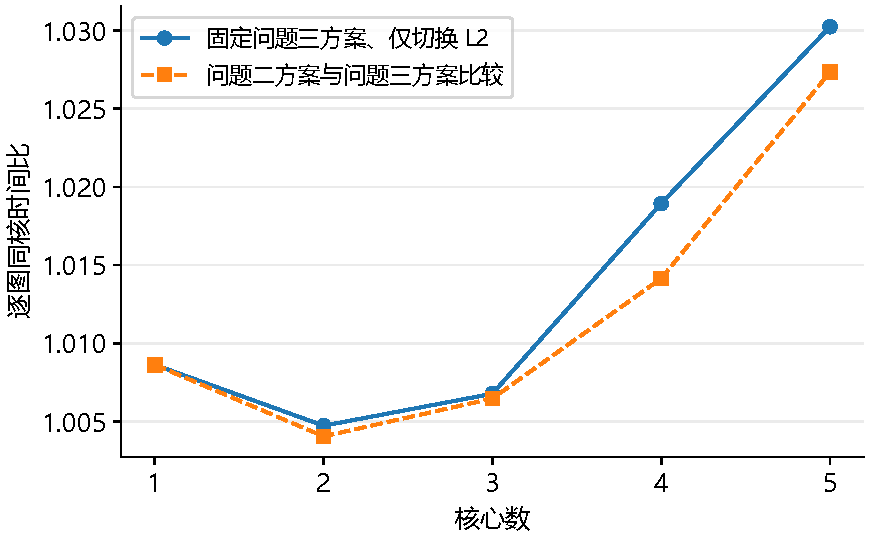
\includegraphics[width=0.85\linewidth,height=0.70\textheight,keepaspectratio]{../图表/runs/20260926-A-q123-complete-delivery/cache_gain.pdf}
\caption{固定问题三方案的 L2 效应与跨方案综合比较}\label{fig:q3-gain}
\end{figure}
问题三五核总额外逻辑搬运为 $1\,150\,596\,866$ 字节。附录的同方案无 L2 与 L2 两次评价采用同一逻辑搬运口径，不从额外搬运中扣除命中字节。命中率并不单独决定周期：FIFO 淘汰、并发冷读、双带宽竞争与数据释放的改变均会影响关键路径。
